\documentclass[10pt,twocolumn,letterpaper]{article}

\usepackage{statcourse}
\usepackage{times}
\usepackage{epsfig}
\usepackage{graphicx}
\usepackage{amsmath}
\usepackage{amssymb}
\usepackage{multirow}
\usepackage{caption}
\captionsetup[table]{skip=7pt}
\usepackage{url}

% Include other packages here, before hyperref.

% If you comment hyperref and then uncomment it, you should delete
% egpaper.aux before re-running latex.  (Or just hit 'q' on the first latex
% run, let it finish, and you should be clear).
\usepackage[breaklinks=true,bookmarks=false]{hyperref}


\statcoursefinalcopy


\setcounter{page}{1}
\begin{document}


%%%%%%%%%%%%%%%%%%%%%%%%%%%%%%%%%%%%%%%%%%%%%%%%%%%%%%%%%%%%%%%
% DO NOT EDIT ANYTHING ABOVE THIS LINE
% EXCEPT IF YOU LIKE TO USE ADDITIONAL PACKAGES
%%%%%%%%%%%%%%%%%%%%%%%%%%%%%%%%%%%%%%%%%%%%%%%%%%%%%%%%%%%%%%%



%%%%%%%%% TITLE
\title{The COVID-19 Face Mask Image Classification}

\author{Christine Hou\\
{\tt\small chou37@wisc.edu}
\and
Yue Yin\\
{\tt\small yin58@wisc.edu}
\and
Seanna Zhang\\
{\tt\small szhang577@wisc.edu}
}

\maketitle
%\thispagestyle{empty}



% MAIN ARTICLE GOES BELOW
%%%%%%%%%%%%%%%%%%%%%%%%%%%%%%%%%%%%%%%%%%%%%%%%%%%%%%%%%%%%%%%


%%%%%%%%% ABSTRACT
\begin{abstract}
    The project aims to explore the applicable machine learning model for classifying whether individuals wear the mask appropriately, incorrectly, or did not wear it at all. To process, we download 4559 raw images from Kaggle. We processed the image data set into two representation ways, the raw pixel representation and color representation.  70\% of each data set is used for training, while the remaining 30\% is used for testing. 20\% of the training set in each data set is accounted for validation. We selected K-Nearest Neighbors, Decision Tree, Bagging (with Decision Tree), Random Forest, XGBoost, and Logistic Regression algorithms to train and test. The tuning strategy is used in each algorithm to improve the test accuracy. In addition, We evaluate the model prediction outcome by the F1 Score and McNemar's Test. Consequently, we find that the XGBoost, with a test accuracy of 94.88\%, is the best machine learning model for this project.
\end{abstract}

%%%%%%%%% BODY TEXT

%-------------------------------------------------
\section{Introduction}
%-------------------------------------------------

In December 2019, a new infectious disease, caused by the virus named SARS-CoV-2, was reported in Wuhan, Hubei, China. When the number of cases continued to rise around the world, the Centers for Disease Control and Prevention (CDC) announced the regulation requiring people to wear the mask in crowded outdoor settings and inside the buildings for adequate protection (https://www.cdc.gov/coronavirus/2019-ncov/prevent-getting-sick/about-face-coverings.html) \cite{online}. Currently, everyone is required to wear the mask while entering the buildings, and there is security personnel ensure that the mask is worn correctly. However, we are concerned such manual inspection is inefficient and wasteful of human effort. With the help of machine learning today, we believe that face mask recognition could achieve the goal while saving human resources. 

Wearing masks has become the primary public health measure to prevent the spread of the current COVID-19 pandemic. Indoor spaces, such as malls, schools, and hospitals, require people to wear masks. Such requirement enforcement is often supervised by personnel. As we claimed early, such inspection is inefficient since it requires inspectors to keep their attention on everyone at all times. From our user experience, we found out many cell phones can recognize whether the owner wears a mask and change the unlock option. Inspiring by such observation, we came up with the idea of applying this face mask detection to the public space. By developing such a tool, we aim to reduce the work of personnel and increase the efficiency of scrutinizing mask-wearing, especially correct mask-wearing behavior. It is critical because we may not eradicate the COVID-19 in years, which means people need to wear masks to protect themselves for a long time. In addition, we believe that by ensuring correct mask-wearing behavior with other factors, such as vaccination, we will significantly reduce the spread of COVID-19.

To be precise with our project goal, we intend to discover the most suitable machine learning algorithms to classify whether people are wearing the mask correctly, wearing it incorrectly, or not wearing it at all. Other people with the same idea or interest can build the real-time face mask recognition from our project result. We download 4559 images with three class labels for our project to start. The class labels are balanced distributed in the data set. We then encode each mask-wearing behavior with numbers to represent the classification results: 0 means correct, 1 means incorrect, and 2 means no mask. 

We trained K-Nearest Neighbors, Decision Tree, Bagging (with Decision Tree), Random Forest, XGBoost, and Logistic Regression algorithm to discover the best machine learning classification model for our project. We select two different ways to represent the raw image data: pixel and color features. The pixel feature is stored into raw\_images.csv, and the color feature is saved in features.csv. Therefore, we have two training sections in the project, each accountable for one data set. Following that, we employ 70\% of each data set for training and the remainder for testing. In addition, we employ 20\% of the training set in each data set for validation. The previously described machine learning algorithms are trained using the two features input gathered in the first phase. We test six models on two data sets and use a tuning strategy \texttt{RandomizedSearchCV} to determine the ideal parameters for each model. Then, we compare the test accuracy from the two training sections to find which input feature gives a better classification result. Finally, we use the F1 score and McNemar's Test to pick the most suitable model.
%-------------------------------------------------
\section{Related Work}
%-------------------------------------------------

Indeed, face recognition is a hot topic for research, and many researchers did the studies using different models. In 2003, M.J.Aitkenheada and A.J.S.McDonald developed and tested the neural-network based facial recognition program (FADER—FAce DEtection and Recognition)\cite{Report3}. They used 1000 images of the face and 1000 images without the face as input, and the detection rate is more than 94\%. Three different neural network models were used to train, and the Hebbian (a neuroscientific theory) connection strength adjustment model gave the highest accuracy of 74.1\%.

Also, many intriguing projects use deep learning and machine learning algorithms to conduct face mask recognition. One study \cite{Report1} used Convolutional Neural Networks (CNN), Support Vector Machine (SVM), and K-Nearest Neighbor (K-NN) models to extract deep features. The authors compared accuracy and precision to obtain the most satisfactory model, and the highest classification rate reached 97.1\%.

Another effort in 2019\cite {Report2} is also using machine learning approaches to identify the face mask. The authors used the Viola-Jones algorithm to detect faces from an image. Furthermore, they addressed and used Principal Component Analysis (PCA) algorithm on masked and non-masked face recognition.  

%-------------------------------------------------
\section{Proposed Method}
%-------------------------------------------------

\subsection{K-Nearest Neighbors}
The first model we decide to use is K-Nearest Neighbors (K-NN). It is one of the supervised machine learning algorithms that are easy to implement while achieving high quality classification results. Given the training features $x^{[i]}$ with its corresponding labels $y^{[i]}$, for $i = 1, ..., n$, the K-NN algorithm simply remembers all of the training data and labels. During the fitting step, as we give K-NN algorithm a query point $x^{[q]}$, the algorithm would loop through all training samples and calculate the distance between current data samples and the query point. Finally, it would pick $k$ smallest distance and its corresponding $k$ training samples and decide query point $x^{[q]}$'s label as the most common labels from $k$ training samples.

For our particular problem, we have five hyperparameters for tuning. $k$ is the number of neighbors the algorithm will pick. We also search for optimal distance metrics with the leaf size and power parameter ($p$). The power parameter is particularly used for the Minkowski distance metric. However, when $p = 1$, it is same as using Manhattan distance metric, and when $p = 2$, it is equivalent to Euclidean distance \cite{KNN}. Finally, we also consider the weight function in the K-NN algorithm, which is either to value all points in the neighborhood equally or to weigh the points by inverse proportional to its distance.

\subsection{Decision Tree}
The second model we use for our data set is the Decision Tree. Unlike the K-NN algorithm, it is an eager supervised learning algorithm, which means it tries to learn from training data and construct a generalized target function to predict newly added data. The decision tree utilizes the Divide-and-Conquer algorithm. Starting from the root node, the algorithm splits training samples into different branches based on features that lead to the most significant information gain. It repeats this splitting recursively until the data at each leaf node belongs to the same label, or there is no improvement.

In our case, we have three possible parameters for tuning. We use the Gini information criterion for splitting, but the number of min samples to split and the maximum depth of the tree is unknown for optimizing. Due to our large-scale data set size, our maximum depth searching range is limited up to 20. We also look for optimized value for the minimum impurity decrease. It means the algorithm would split the node if such split causes the impurity to decrease more than the given value \cite{decisionTree}.

\subsection{Ensemble Methods}
As we utilize the Decision Tree classifier on image features, we may wonder which elements lead to more accurate results for splitting. This is a natural idea, as we know that image features on the lips will have different changes due to the presence and absence of the mask. We hope that our model can consider these changes. The ensemble methods would actually allow us to take a set of the decision trees into account and pick the features that are important for prediction. Thus, we decide to use three ensemble methods, Bagging, Random Forest, and XGBoost, to improve the Decision Tree model. 

\subsubsection{Bagging}
Bagging, also called Bootstrap Aggregating, is an ensemble method to fit the base model (in our case, Decision Tree) into random bootstrapped samples from the original data set. Then, we aggregated the predictions from each individual model to build up the final predictor. Due to the size of our image data set, we only consider 50 base estimators in this ensemble method. We also decided to use out-of-bag samples to validate its prediction scores and estimate the generalized error. 

\subsubsection{Random Forest}
Random Forest is another ensemble method we apply to the Decision Tree model. It extends the bagging method that not randomly selects subsets of samples but also the subsets of features for each bootstrapped instance. This randomness helps to make each decision tree more independent and improves the ensemble prediction. For our particular case, we select 100 trees to train and choose three parameters for optimizing: the minimum number of samples to split, the minimum impurity decrease value, and the maximum tree depth. 

\subsubsection{XGBoost}
The final ensemble method we use is XGBoost, which stands for Extreme Gradient Boosting. Precisely, XGBoost is a scalable gradient boosted decision tree machine learning library \cite{XGBoost}. Similar to the random forest, gradient boosting is built from multiple decision trees. The difference is that gradient boosting creates the final predictor from many weak learners through several boosting rounds. The gradient decision tree iteratively trained the new model based on the error residuals from the previous model. It weighted the sum of all the tree predictions until there was no improvement. There are various booster parameters and learning task parameters; the former helps the booster while the latter one decides the learning scenario \cite{XGBoostDoc}. We let the random search tuning strategy help us find the best combination of these parameters. 

\subsection{Logistic Regression}
Finally, we have our last model, Logistic Regression. It is a classical and widely used algorithm for classification. Specifically, we use multinomial logistic regression to generalize the logistic regression with three classes. The difference between logistic regression and other classification algorithms is that logistic regression calculates the probability of categorical membership by estimating the maximum likelihood. 

The multinomial logistic regression is generalized from binary logistic regression. Explicitly, the model formula we would use is $$P(Y_i = k) = \frac{\exp{(\beta_{0k} + x_{i}\beta_{k}^{'})}}{\sum_{j = 1}^{m}\exp{(\beta_{0j}+x_{i}\beta_{j}^{'})}}$$
where x is the set of features and Y is the label. $\beta_{k}$ is the coefficients vector of X for the $k$th category of Y. In our case, we are estimating the probabilities for $m = 3$ categories \cite{multinomial}. These unknown coefficients vector is estimated by minimizing the negative log likelihood $$\sum_{i = 1}^{N}\sum_{k = 1}^{M}-y_{k}^{[i]}\log{(a_{k}^{[i]})}$$
where N is the training sample size, M denotes the number of groups (labels), $x_{k}^{[i]}$ represents the features of the $i$th sample with $k$th label (group $k$) in the training set, $y_{k}^{[i]}$ denotes the corresponding label. a is the activation function output $$h(x) = \sigma{(\beta^{T}x + \beta_{0})} = a$$ \cite{lec_note}
%-------------------------------------------------
\section{Experiments}
%-------------------------------------------------

This section presents the information about our data set, software, and hardware. Since this project is based on the analysis of images, we also demonstrate our step to process the raw image data to make it practical for our model training.

\subsection{Dataset}

The dataset we choose is from Kaggle named "Face-Mask Recognition Dataset (FMRD)" (link: https://www.kaggle.com/hadjadjib/facemask-recognition-dataset) \cite{FMRD}. It consisted of 4559 images with three class labels, "Correct," "Incorrect," and "NoMask." The Table\ref{raw_data} shows the raw data structure of FMRD.

\begin{table}[!htbp]
\centering
\begin{tabular}{|l|c|}
\hline
Label & Count \\
\hline\hline
Correct & 1559 \\
Incorrect & 1500 \\
NoMask & 1500 \\
\hline
Total & 4559 \\
\hline
\end{tabular}
\caption{This is the raw data structure of image data set}
\label{raw_data}
\end{table}

According to the table, the data from FMRD are generally balanced, so we simply do a stratification split after the data processing to make sure each training, validation, and test set would have balanced class labels. The data processing steps will be explained in the following subsection. The ratio of training, validation, and test dataset are 0.56:0.14:0.30.

\subsection{Data Processing}
Before we are able to train any practical machine learning algorithm, we need to transform the input image into a vector of some numbers that represent the contents of the picture. We first simply take the input image, resize it to a fixed size, and then flatten three color channel components into one single array input. In other words, this is simply a raw pixel representation. The data was processed and stored into file "raw\textunderscore image.csv" for later training. The overall size after transformation is 3.42 GB. Since this representation leads to a large data size, we also try another representative method, hoping to get a good result while saving running time. The other representation is the color histogram, coming from the idea that the color of the mask and human face would be different, so the image's color distribution may be an appropriate feature for training. This transformation has a much better storing size, 58.4 MB. The data is stored in file "features.csv." At the same time, we also save labels information into the file "labels.csv." We then read all data information from these three csv files and train the data.

\subsection{Software}

For the data processing and model training, we simply use Jupyter Notebook with Python 3.8 or 3.9, depending on each of our systems. We have used NumPy and Pandas for data processing, reading, and splitting, matplotlib and mlxtend for plotting the graph we need, scipy for general computing, and scikit-learn and xgboost for various model training. 

\subsection{Hardware}

Each group member uses their own laptop, all for Mac with different chips.

%-------------------------------------------------
\section{Results and Discussion}
%-------------------------------------------------

After processing the images we access online, we obtain the images into a $4559\times30000$ matrix for pixel representation and a $4559\times512$ matrix for color representation. We use \texttt{train\_test\_split} to divide each of two data into 70\% of training and 30\% of testing, and use \texttt{train\_test\_split} again to obtain 20\% of training set as validation set. The split is stratified to make sure that training, testing, and validation sets can have the same proportions of 0 (correct), 1 (incorrect), and 2 (no mask) as observed in the original data. For randomness, we use the random seed of 123. To conduct the hyperparameter tuning, we choose \texttt{RandomizedSearchCV}. 

We trained and tuned models on both input features and compared their accuracy results. Table \ref{comparison} shows the comparison. According to the table, we find out that the relatively large dataset raw\_images.csv has higher accuracy in general, so for convenience and length of report, we will only present our training and tuning process on pixel representation in the following sections.

\begin{table}[!htbp]
\centering 
\begin{tabular}{|c|c|c|}
\hline
Models & features.csv & raw\_images.csv \\
\hline\hline
K-NN &  83.26\% & 92.62\% \\
Decision Tree &  87.21\% & 90.13\%\\
Bagging & 89.18\% & 91.23\% \\
Random Forest &  90.72\% & 94.44\% \\
XGBoost & 91.74\% & 94.88\% \\
Logistic Regression &  78.22\% & 93.20\% \\
\hline
\end{tabular}
\caption{Accuracy Comparisons on Two Input Features}
\label{comparison}
\end{table}


\subsection{Training and Hyperparameter Tuning}
\subsubsection{K-NN}

We use \texttt{KNeighborsClassifier} to build the K-NN model. Two parts are involved in finding the best parameter $k$ and the other parameters for the model. Firstly, we compare each error rate corresponding to $k$ and choose the parameter $k$ with the lowest error rate. We examine $k$ from 1 to 29 and compute the corresponding error rates. From Figure \ref{KNN}, we can see that the lowest error rate occurs when $k$ is 4, and the error rate increases when $k$ is larger than 4. Therefore, using the error rate, we train the K-NN model with $k = 4$ with $p = 2$ (euclidean\_distance) and uniform weight function. This model is the base K-NN model.

\begin{figure}[!htbp]
\begin{center}
   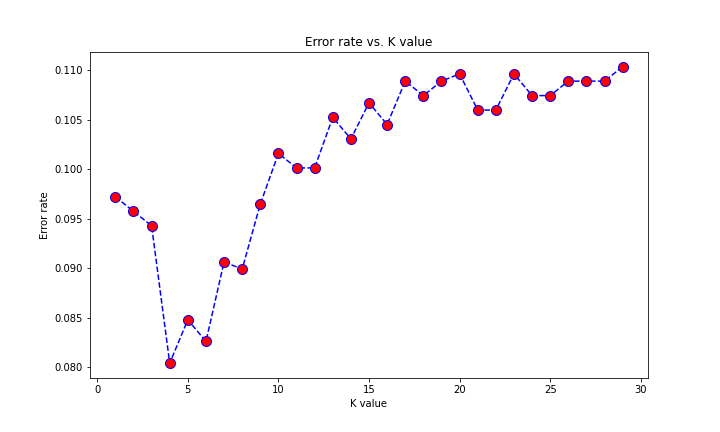
\includegraphics[width=1\linewidth]{Figures/KNN-Input 2.png}
\end{center}
\vspace{-0.5cm}
   \caption{KNN - Error Rate vs. Neighbours}
\label{KNN}
\end{figure}

Then, we use the tuning strategy to explore parameters that produce a better performance of the K-NN model. Five parameters are involved in the tuning process: the number of neighbors, leaf size, power parameter ($p$), weight function (weights), and distance metric to use for the model (metric). Based on the error rate we checked before, we only search for the optimal value of $k$ from 3 to 7 because larger $k$ has a larger error rate, which may not work well for the model. In addition, we set leaf size from 20 to 31 coupling with $p$ = [1,2], weights = [`uniform',`distance'] and metric = [`minkowski',`chebyshev']. After tuning, we get the best parameter for the K-NN model shown in the Table \ref{KNN-tuning}. 

\begin{table}[!htbp]
\centering
\begin{tabular}{|c|c|c|c|c|}
\hline
n\_neighbors & leaf\_size & p & weights    & metric      \\ \hline
6            & 20         & 1 & `distance' & `minkowski' \\ \hline
\end{tabular}
\caption{Best Parameters in K-NN Model}
\label{KNN-tuning}
\end{table}

Using the K-NN model from the error rate method, we obtain its test accuracy of 91.96\%. When we further apply the tuning strategy, we get the test accuracy of 92.62\%. We see an increase in test accuracy, so we use the model with 92.62\% for future accuracy comparison. Its F1 score is equal to 0.9263.

\subsubsection{Decision Tree}

We use \texttt{DecisionTreeClassifier} for the Decision Tree Model. Without tuning strategy, the parameters are default with the random seed of 123, and we get the test accuracy of 87.87\%. Then, we apply the tuning strategy. There are three hyperparameters involved: max\_depth, min\_sample\_split, and min\_impurity\_decrease. We search for the optimal max\_depth from 1 to 20 coupling with min\_sample\_split from 2 to 11 and min\_impurity\_decrease from 0 to 0.5. Finally, we find the best parameters shown in the Table \ref{Decision Tree}.

\begin{table}[!htbp]
\centering
\begin{tabular}{|c|c|c|}
\hline
min\_samples\_split & min\_impurity\_decrease & max\_depth \\ \hline
2                   & 0.011493972900871952   & 4       \\ 
\hline
\end{tabular}
\caption{Best Parameters in Decision Tree}
\label{Decision Tree}
\end{table}

After tuning, the Decision Tree model produces the test accuracy of 90.13\%, and we also compute its F1 score equal to 0.9018.

\subsubsection{Bagging on Decision Tree}
By using \texttt{BaggingClassifier} from scikit-learn, we want to apply bagging to the previous best decision tree to improve its performance. Considering the size of our dataset, we only use 50 base estimators, and the other parameters are as shown in Table \ref{Bag}:

\begin{table}[h]
\centering
\begin{tabular}{|c|c|c|c|}
\hline
oob\_score & bootstrap & bootstrap\_features & n\_jobs \\ \hline
True       & True      & False               & 1      \\ \hline
\end{tabular}
\caption{Tuning Parameters in Bagging}
\label{Bag}
\end{table}

The test accuracy is slightly improved to reach 91.23\%, as well as the 0.9121 F1 score, so the ensemble method has some positive effect on the performance of the decision tree.

\subsubsection{Random Forest}

For Random Forest, we use \texttt{RandomForestClassif\newline ier} with 100 estimators and a random seed of 123 to build the model without tuning strategy, and it achieves the test accuracy of 94.44\%. To check whether the model after tuning can have higher test accuracy, we do similar works to Decision Tree that there are three hyperparameters involved: max\_depth, min\_sample\_split, and min\_impurity\_decrease. We search for the optimal max\_depth from 1 to 20 coupling with min\_sample\_split from 2 to 11 and min\_impurity\_decrease from 0 to 0.5. Finally, we find the best parameters shown in the Table \ref{Random Forest}.

\begin{table}[!htbp]
\centering
\begin{tabular}{|c|c|c|}
\hline
min\_samples\_split & min\_impurity\_decrease & max\_depth \\ \hline
15                   & 0.013666043770271419   & 2       \\ 
\hline
\end{tabular}
\caption{Best Parameters in Random Forest}
\label{Random Forest}
\end{table}

After tuning, the Random Forest model produces the test accuracy of 90.42\%. The model with tuning has lower test accuracy than the model without adjusting, so we decide to use the model with the test accuracy of 94.44\% as our final Random Forest model for future algorithm comparison. Additionally, we compute its corresponding F1 score, equal to 0.94438.

It's normal to see that the Random Forest model has higher test accuracy than the Decision Tree model. The random forest relies on assembling many decision trees to arrive at its final predictor. This aggregation usually improves the weak prediction happening in a single decision tree. Even though the Decision Tree is easier to understand, Random Forest works better on the large dataset such as our input. The ensemble algorithms, including the other classifiers (bagging, xgboost), are more robust than a single decision tree. 

\subsubsection{XGBoost}
For XGBoost, we use the \texttt{XGBClassifier} from xgboost package. We tune 12 hyperparameters such as n\textunderscore estimators and alpha. The exact values for each parameter are shown in the Table \ref{XGBoost}. 

\begin{table}[!htbp]
\centering
\begin{tabular}{|c|c|}
\hline
Hyperparameter  & Value Range                      \\ \hline
\hline
n\_estimators     & 30, 50, 100, 300, 500             \\ \hline
min\_child\_weight & 4,5                               \\ \hline
reg\_lambda       & $10^{-8}$ - 1                         \\ \hline
alpha            & $10^{-8}$ - 1                         \\ \hline
gamma            & 0.3 - 0.6                           \\ \hline
subsample        & 0.6 - 1.1                           \\ \hline
colsample\_bytree & 0.6 - 1.1                           \\ \hline
max\_depth        & 2,3,4,6,7                         \\ \hline
objective        & `reg:squarederror', `reg:tweedie' \\ \hline
booster          & `gbtree', `gblinear'              \\ \hline
eval\_metric      & `rmse'                            \\ \hline
eta              & 0.3 - 0.6                           \\ 
\hline
\end{tabular}
\caption{Tuning Parameters in XGBoost}
\label{XGBoost}
\end{table}

Due to the large size of both dataset and hyperparameters, we use random search \texttt{RandomizedSearchCV} to find the best hyperparameters out of 15 iterations of 5-fold cross validation to make it less expensive. After tuning, we found the best hyperparameters, and they are shown in Table \ref{XGBoost2}.

\begin{table}[!htbp]
\centering
\begin{tabular}{|c|c|}
\hline
Hyperparameter  & Value                      \\ \hline
\hline
n\_estimators     & 500             \\ \hline
min\_child\_weight & 4                             \\ \hline
reg\_lambda       & 0.0576480249714419                         \\ \hline
alpha            & 0.3929444207680876                         \\ \hline
gamma            & 0.5                           \\ \hline
subsample        & 1.0                           \\ \hline
colsample\_bytree & 1.0                           \\ \hline
max\_depth        & 2                         \\ \hline
objective        & `reg:squarederror' \\ \hline
booster          & `gbtree'              \\ \hline
eval\_metric      & `rmse'                            \\ \hline
eta              & 0.3                           \\ 
\hline
\end{tabular}
\caption{Best parameters in XGBoost}
\label{XGBoost2}
\end{table}

The after-tuning model has a test accuracy of 94.88\% and an F1 score of 0.9487.

\subsubsection{Logistic Regression}
We import \texttt{LogisticRegression} from scikit-learn library. The tuning strategy changes the $L_1$ regularization parameter C, the boolean value to decide if added a constant term to the decision function (fit\_intercept), and a boolean value to decide whether to use the previous solution (warm\_start) (Table \ref{Regression}). 

\begin{table}[h]
\centering
\begin{tabular}{|c|c|}
\hline
Hyperparameter & Value Range                  \\ \hline
C              & scipy.stats.expon(scale=.01) \\ \hline
fit\_intercept & True, False                  \\ \hline
warm\_start    & True, False                  \\ \hline
\end{tabular}
\caption{Tuning Parameters in Logistic Regression}
\label{Regression}
\end{table}

After doing a random search of 15 iterations with 5-fold cross-validation, we find the best hyperparameters shown in Table \ref{LR}.

\begin{table}[h]
\centering
\begin{tabular}{|c|c|c|}
\hline
C        & fit\_intercept & warm\_start \\ \hline
0.002573 & True           & False       \\ \hline
\end{tabular}
\caption{Best Parameters in Logistic Regression}
\label{LR}
\end{table}

The model using the best hyperparameters achieves a test accuracy of 93.20\% and an F1 score of 0.9320.

\subsection{Model Evaluation and Selection}

\subsubsection{McNemar's Test on Random Forest and XGBoost}
Since the performances of the random forest and XGBoost models are best according to the F1 score, we use McNemar's Test to check whether these two models have the same results for our particular problem. Our null hypothesis is that the performances of the two models are equal. Figure \ref{Forest}, Figure \ref{Boost}, and Table \ref{CM} show some details.

\begin{table}[!htbp]
\centering
\begin{tabular}{llll}
                             &                              & \multicolumn{2}{l}{Random Forest}                         \\ \cline{2-4} 
\multicolumn{1}{l|}{}        & \multicolumn{1}{l|}{}        & \multicolumn{1}{c|}{correct} & \multicolumn{1}{c|}{wrong} \\ \cline{2-4} 
\multicolumn{1}{c|}{XGBoost} & \multicolumn{1}{c|}{correct} & \multicolumn{1}{c|}{1277}    & \multicolumn{1}{c|}{15}    \\ \cline{2-4} 
\multicolumn{1}{l|}{}        & \multicolumn{1}{c|}{wrong}   & \multicolumn{1}{c|}{21}      & \multicolumn{1}{c|}{55}    \\ \cline{2-4} 
\end{tabular}
\caption{Confusion Matrix - XGBoost \& Random Forest}
\label{CM}
\end{table}

\begin{figure}[!htbp]
\begin{center}
   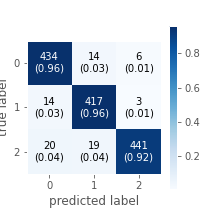
\includegraphics[width=0.5\linewidth]{Figures/forest_cm.png}
\end{center}
\vspace{-0.5cm}
   \caption{McNemar's Test - Random Forest}
\label{Forest}
\end{figure}

\begin{figure}[!htbp]
\begin{center}
   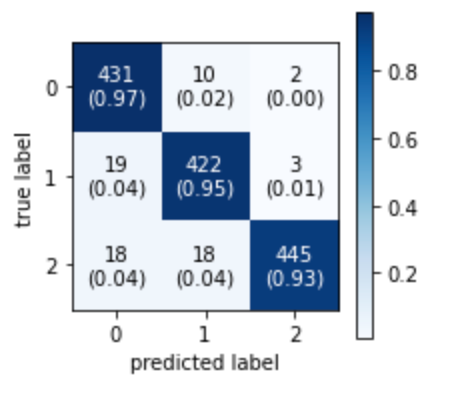
\includegraphics[width=0.5\linewidth]{Figures/XGBoost-cm.png}
\end{center}
\vspace{-0.5cm}
   \caption{McNemar's Test - XGBoost}
\label{Boost}
\end{figure}

The p-value we get from the test is 0.4047, which is greater than $\alpha=0.05$, so we fail to reject the null hypothesis and conclude that the performances of the two models are the same. Thus, based on Figure \ref{F1score}, we will choose the model with the slightly higher F1 score as our final model--XGBoost.

\begin{table}[!htbp]
\centering
\begin{tabular}{|c|c|}
\hline
Random Forest& XGBoost \\ \hline
0.94438 & 0.9487 \\ 
\hline
\end{tabular}
\caption{F1 Score Comparison}
\label{F1score}
\end{table}

\subsection{Discussion}

Although we achieve a high accuracy in two models, it is extremely computationally expensive to fit the models and tune the hyperparameters due to the large size of our dataset, which will be one of the weaknesses of our project. In addition, we separate our dataset into training, test, and validation datasets, which may lead to a pessimistic bias in our result. Future improvement can include other different feature representations, such as features of shape or texture, which may reduce the number of input variables while achieving high prediction results and saving the cost.

At the same time, we acknowledge that Convolutional Neural Networks (CNN) is a robust model for image classification. Due to the time limit, we haven't had a chance to try CNN in our data set. If any other who have a similar interest in face mask recognition, we believe CNN would be a worthy option for a try. 

%-------------------------------------------------
\section{Conclusions}
%-------------------------------------------------

\begin{figure}[!htbp]
\begin{center}
   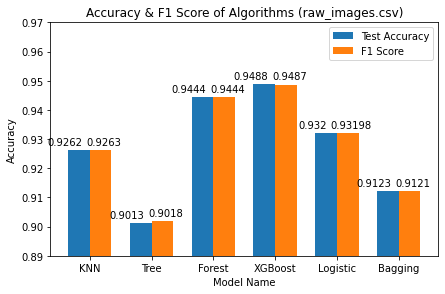
\includegraphics[width=1\linewidth]{Figures/Accuracy vs. F1 Score.png}
\end{center}
\vspace{-0.6cm}
   \caption{Test Accuracy \& F1 Score}
   \label{score}
\end{figure}

We have accomplished our initial motivation in the above analysis by finding the optimal way to classify images of people wearing masks, not wearing masks, and wearing masks incorrectly. We investigate six potential algorithms, including K-NN, Decision Tree, Bagging, Random Forest, XGBoost, and Logistic Regression. We train them on the training dataset and tune hyperparameters using random search. Finally, we evaluate different models using both test accuracy and F1 score, and compare the best two models Random Forest and XGBoost by McNemar's Test. We conclude that XGBoost with an F1 score of 0.9487 will be our final model, although Random Forest has the same good performance. All the accuracy and F1 scores are shown in the Figure \ref{score} above.

We aim to efficiently scrutinize mask-wearing behavior during the pandemic to protect public health. We hope to improve our classification algorithm to make it less computationally expensive in the future. It would be appreciated and excited if other people engaging in real-time face mask recognition could utilize our classification model and apply it to public places such as malls and airports in the future. 
%-------------------------------------------------
\section{Acknowledgements}
%-------------------------------------------------

We give many thanks to user \textit{hadjadji b} on Kaggle for publishing the face mask dataset and allowing unrestricted use of them.

%-------------------------------------------------
\section{Contributions}
%-------------------------------------------------

Seanna Zhang found the original image dataset online, extracted the feature datasets, and cleaned up the data for further analysis. Christine Hou trained and evaluated the K-NN, Decision Tree, and Random Forest models with hyperparameter tuning. Yue Yin trained and assessed the rest models-- XGBoost, Logistic Regression, and Bagging on Decision Tree, and did the McNemar's Test.

For the report, Seanna wrote the Proposed Method and Experiments section. Christine finished the Abstract, Introduction, Related Work, and Results and Discussion part. Yue Yin completed the rest of the Results and Discussion, Conclusions, Acknowledgements, and Contributions.


{\small
\bibliographystyle{ieee}
\bibliography{bibliography.bib}
}

\end{document}
